% Template for ISBI-2016 paper; to be used with:
%          spconf.sty  - ICASSP/ICIP LaTeX style file, and
%          IEEEbib.bst - IEEE bibliography style file.
% --------------------------------------------------------------------------
\documentclass{article}
\usepackage{spconf,amsmath,graphicx}
\usepackage{amsfonts}
\usepackage[utf8]{inputenc}
\usepackage[francais]{babel}
%\usepackage{hyperref}
\PassOptionsToPackage{hyphens}{url}\usepackage{hyperref}
% Example definitions.
% --------------------
\def\x{{\mathbf x}}
\def\L{{\cal L}}

% Title.
% ------
\title{Nuclei Segmentation in Histopathology
  images using Deep Neural Networks}
%
% Single address.
% ---------------
%%% Not too sure about who to thank, I guess me, you, phil, and ema?
%\name{Peter Naylor, Marick Lae, Fabien Reyal and Thomas Walter\thanks{}}
%\address{(1)   MINES ParisTech, PSL Research University, CBIO - Centre de bio-informatique, 35 rue St Honoré 77300 Fontainebleau, France
%(2)   Institut Curie, 75248 Paris Cedex, France
%(3)   INSERM U900, 75248 Paris Cedex, France}
%
% For example:
% ------------
%\address{School\\
%	Department\\
%	Address}
%
% Two addresses (uncomment and modify for two-address case).
% ----------------------------------------------------------
%\twoauthors
%  {A. Author-one, B. Author-two\sthanks{Thanks to XYZ agency for funding.}}
%	{School A-B\\
%	Department A-B\\
%	Address A-B}
%  {C. Author-three, D. Author-four\sthanks{The fourth author performed the work
%	while at ...}}
%	{School C-D\\
%	Department C-D\\
%	Address C-D}
%
% More than two addresses
% -----------------------

\name{Peter Naylor$^{1,2,3}$\sthanks{Peter Naylor has received a PhD
  fellowship from the Ligue contre le Cancer} \qquad Marick La\'e$^{4}$
  \qquad Fabien Reyal$^{5,6,7}$\qquad Thomas Walter$^{1,2,3}$}

\address{\normalsize $^{1}$MINES ParisTech, PSL Research University, CBIO - Centre
  de Bioinformatique, 77300 Fontainebleau, France;\\
\normalsize $\quad ^{2}$Institut Curie,  
$\quad ^{3}$INSERM U900, Paris, 
$\quad ^{4}$Service de Pathologie, Institut Curie, Paris, F-75248, France\\
\normalsize $\quad ^{5}$Residual Tumor \& Response to Treatment Laboratory,
RT2Lab, Translational Research Department, Institut Curie, \\
\normalsize $\quad ^{6}$U932, Immunity and Cancer, INSERM, Institut Curie, 
$\quad ^{7}$Department of Surgery, Institut Curie, Paris, F-75248, France.
}
%

\begin{document}
%\ninept
%
\maketitle

%
\begin{abstract}
Analysis and interpretation of stained tumor sections is one of the
main tools in cancer diagnosis and prognosis, which is mainly carried
out manually by pathologists. The avent of digital pathology provides
us with the challenging opportunity to automatically analyze large
amounts of these complex image data in order to draw
biological conclusions from them and to study cellular and tissular
phenotypes at a large scale. One of the bottlenecks for such
approaches is the automatic segmentation of cell nuclei from this type
of image data. Here, we present a fully automated workflow to segment
nuclei from histopathology image data by using deep neural
networks trained from a set of manually annotated images and by processing
the posterior probability maps in order to split jointly segmented
nuclei. Further, we provide the image data set that has been generated
for this study as a benchmark set to the scientific community.  
\end{abstract}
%
\begin{keywords}
Deep Learning, Convolutional Neural Networks, Nuclei Segmentation,
Histopathology, Digital Pathology, Breast Cancer, Cellular Phenotyping
\end{keywords}
%
\section{Introduction}
\label{sec:intro}

% images in cancer research, histopathology --> digital pathology
\noindent Today, large sequencing approaches build the main body of cancer
research programs and they have revolutionized our understanding of
the molecular basis of cancer. In clinical practice however,
molecular profiling is paralleled with the more traditional
(and mostly manual) analysis of stained histological tumor
sections. With the avent of digital pathology, i.e. the scanning and
digital storage of diseased tissue sections, it is now possible to
build tools for the quantitative and automatic analysis of these
complex and informative image data, which are complementary to genomic
and expression data.

%These image data are in many ways
%complementary to genomic and expression data, as they are informative
%about the spatial dimension, they allow one to assess cellular
%heterogeneity and they enable single cell analysis in terms of
%morphology and phenotype. 


% two approaches: CAD vs. understanding, importance of segmentation
For these reasons, analysis of histopathology data has received much
attention over the last years. In particular for approaches aiming at
relating biologically relevant features (such as phenotype
distributions or heterogeneity measures) to clinical variables,
segmentation of nuclei from tissue images is essential. 

%While many approaches aim at
%automatically performing the task of a human pathologist (Computer
%Aided Diagnosis, CAD), we want to investigate the influence of
%biologically relevant features, such as phenotype distributions or
%heterogeneity measures from the tissue data on different clinical
%variables, such as resistance to treatment or relapse probability.
%One essential step is thus the segmentation of nuclei from tissue
%images,  in order to assign them a cell type or phenotypic label and
%to evaluate their spatial distribution.

%Most of these works are in the frame of
%Computer Aided Diagnosis (CAD) and aim at automatically performing the
%task of a human pathologist or at assisting in the diagnosis. For such
%a task, the nature of the features according to which a certain
%classification or detection task is solved is mostly
%irrelevant. A conceptually different approach is to derive biologically
%relevant features, such as phenotype distributions, spatial cell type
%distributions or heterogeneity measures from the tissue data in order to reach some
%understanding as of which biological features can be predictive for
%clinical variables such as resistance to treatment or relapse
%probability. 

% segmentation is the bottleneck of cellular phenotyping in cancer
% tissues. 
%In this latter case, one of the essential steps is to
%segment nuclei from tissue images in order to be able to
%assign them a cell type or phenotypic label and to evaluate their
%spatial distribution. We concentrate on nuclei, as they are indicative
%of many cellular phenotypes\cite{Chow2012}, and their morphology is 
%currently used by pathologists in order to
%identify the mitotic index and the level of nuclear
%pleomorphism\cite{Elston1991}. 

However, segmentation of nuclei is a
complicated task: tissue type, staining differences and cell type
convey them different visual characteristics, which makes it very difficult to
design traditional image segmentation algorithms that work
satisfactorily for all of these different cases. On the other hand,
deep learning algorithms have been used recently with great success to
complex segmentation tasks in biology\cite{Ciresan2012,UNet}. 

The contribution of this paper is three-fold: (1) we generated a
set of manually annotated, representative images containing segmentation results for
more than 2000 cells. We believe that such datasets
can trigger methodological developments and are
important for the field. (2) We apply a deep neural network end-to-end strategy and
demonstrate the superiority of this approach with respect to
previously proposed simpler architectures. (3) We propose a
post-processing strategy of the posterior probabilities provided by
the network. This approach is based on mathematical
morphology and unlike many adhoc procedures allows a clearly defined
and intuitive criterion for the object splits.

\section{Related work}
\label{sec:related}

\noindent Many traditional techniques have been proposed for the segmentation of
nuclei in histopathology images, ranging from simple background
subtraction and color threshold techniques 
to much more
sophisticated approaches, such as marked point
processes\cite{Kulikova2012}. Many of these methods have been recently
reviewed \cite{irshad2014methods}.    

%Image segmentation and object recognition in medical imaging have 
%been tackled for many years and many approaches have been proposed. 
%Methods based on mathematical morphology have been 
%widely used and applied for segmentation and feature extraction, 
%however such methods rely on the user to manually define the 
%information that is relevant for his task \cite{irshad2014methods}. 
%Segmentation methods based on a strong priori information are also 
%possible and yield comparable results in terms of accuracy, in 
%\cite{ranefall2016fast} they segment the picture using mathematical 
%morphology with an ellispe fit condition 
%which is considerably faster than other state of the art methods. 
%Graph-
%based tools for segmentation are also possible in histopathology 
%\cite{ta2009graph}. 
%\cite{manivannanlocal} focus on gland 
%segmentation, they achieve good results by predicting image patches as 
%a whole, via a classification scheme. The output confidence vector is 
%then preprocessed to obtain the final segmentation. 

Alternative methods 
have arisen from the achieving Convolutional neural networks.
%\cite{lecun}, 
%in particular strong incentive rose with the very impressive 
%results that they achieved in the pascal voc challenge with 
%\cite{ImageNet}. 
Recent advances in deep neural networks, and in 
particular in their optimization have made them become the state-of-the-
art model for object recognition.  Deep neural network have also been 
used for 
semantic segmentation, where \cite{long2015fcn} use "de-
convolution layers" and up-sampling in order to identify and precisely 
locate objects within a picture. Different architecture arising from 
different intuition are also possible and have been applied in this paper.

Learning based methods rely on annotated data sets. But for the
problem of nuclei segmentation in histopathology images, there are
only few manually segmented images freely available. 
In \cite{Drelie08-298}, a partially annotated data set has been
released. However, this data set does not cover the morphological
variability typically encountered in real histopathology data. 

\begin{figure}[htb]
\begin{minipage}[b]{.48\linewidth}
  \centering
  \centerline{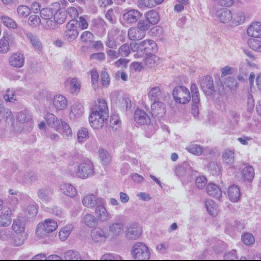
\includegraphics[width=4.0cm]{RGB_1}}
%  \vspace{1.5cm}
  \centerline{Sample from patient 498959}\medskip
\end{minipage}
\hfill
\begin{minipage}[b]{0.48\linewidth}
  \centering
  \centerline{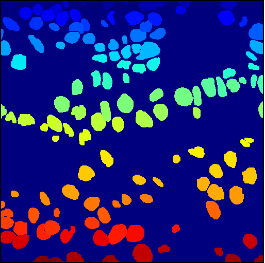
\includegraphics[width=4.0cm]{GT_1}}
%  \vspace{1.5cm}
  \centerline{Associated ground truth}\medskip
\end{minipage}
%
%
%\begin{minipage}[b]{.48\linewidth}
 % \centering
%  \centerline{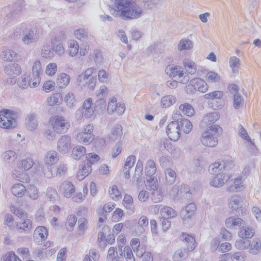
\includegraphics[width=4.0cm]{RGB_2}}
%  \vspace{1.5cm}
%  \centerline{Sample from patient 581910}\medskip
%\end{minipage}
%\hfill
%\begin{minipage}[b]{0.48\linewidth}
%  \centering
%  \centerline{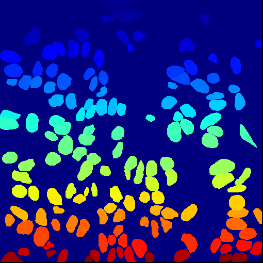
\includegraphics[width=4.0cm]{GT_2}}
%  \vspace{1.5cm}
%  \centerline{Associated ground truth}\medskip
%\end{minipage}
%
%
\begin{minipage}[b]{.48\linewidth}
  \centering
  \centerline{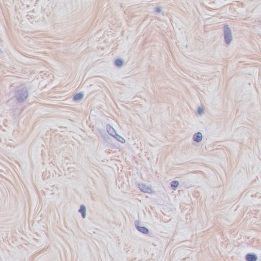
\includegraphics[width=4.0cm]{RGB_3}}
%  \vspace{1.5cm}
  \centerline{Sample from patient 581910}\medskip
\end{minipage}
\hfill
\begin{minipage}[b]{0.48\linewidth}
  \centering
  \centerline{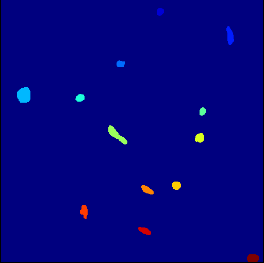
\includegraphics[width=4.0cm]{GT_3}}
%  \vspace{1.5cm}
  \centerline{Associated ground truth}\medskip
\end{minipage}
%
\caption{Random annotated samples from the dataset}
\label{fig:annotation}
%
\end{figure}


\section{Data set}
\label{sec:dataset}

%% Contribution as a dataset, small introduction
\noindent One of the contributions of this paper is the now publicly available 
nuclei detection dataset within HE stained histopathology images which 
can be found at \url{http://cbio.mines-paristech.fr/~pnaylor/BNS.zip}. This annotated dataset provides images clustered by 
patients. Each patient has at least 3 annotated $512 \times 512$ HE 
histopathology images with their associated ground truth. Each 
ground truth image is a $512 \times 512$ label image where each pixel value above 
$0$ is considered as the label of the corresponding nucleus. 
See figure \ref{fig:annotation} for an example of 
three annotated images. This annotation was conducted via the help of 
the software ITK-snap, \cite{py06nimg} \url{http://www.itksnap.org} by
the authors of this paper. 



%% Data set creation procedure
The patients were randomly picked from an unpublished study on
triple negative breast cancer (TNBC). For each of the patients we had access
to a biopsy and a whole slide image (WSI). WSI are very large images
and can be up to 60 GB 
(uncompressed). As they cannot be stored in the RAM of a standard computer, we randomly cropped $512 \times 512$ samples 
from the WSI. %% explain that we choose the tissue area? 
3 to 7 images were choosen from the randomly sampled images to try and
give the most diverse dataset among these patients. Once the samples
were choosen, we fully annotated each nucleus via the software
ITK-snap; touching nuclei were differentiated by the different label
value. 

%%Data set description 
%% I asked Marick's help for this paragraph!
In this data set we have annotated a considerable amount of cells,
including normal epithelial and myoepithelial breast cells (localized in
ducts and lobules), invasive carcinomatous cells, fibroblasts, endothelial
cells, adipocytes, macrophages and
inflammatory cells (lymphocytes and plasmocytes). For the moment, we
did not annotate the different cell types, however. 

In total, we have 33 images with a total of 2754 annotated cells,
the maximum number of cells in one sample is 293 and the minimum
number of cells in one sample is 5. We also have on average 83 cells
per sample with a high standard deviation of 63. 

% \begin{itemize}
% \item Number of images: 33 \\
% \item Number  of cells: 2754 \\
% \item Maximum number of cells in one sample: 293 \\
% \item Minimum number of cells in one sample: 5 \\
% \item Mean number of cells: 83 \\
% \item Standard deviation of number of cells: 63 \\
% \end{itemize}

\section{Methodology}
\label{sec:method}
%% Segmentation task
\noindent Let A be the space of RGB images, A can typically be 
$\mathbb{R}^{n \times p \times 3}$ and let B the space B the space of annotation 
images, in our case $\{0,1\}^{n \times p}$. We have a set of 
$(A_l,B_l)_{l \in [1, N]}$ for a supervised learning approach. Our goal is 
a prediction task 
named as semantic segmentation, we wish to maximize the prediction of 
an unseen element belonging to B given an new element in A. We maximize 
thus prediction by modelizing our prediction function as the softmax output of a deep neural 
network. We find the model parameters by minimizing a log loss function 
defined as:
 $\frac{1}{\sum_{i,j}w_{ij}} \sum_{i,j} \sum_k w_{i,j} t_{i,j,k} \log (\widehat{p_{i,j,k}})$
, where $k$ designates a certain label, $w_{i,j}$ is a 
certain weight given to pixel $i,j$, $t_{i,j,k}$ is equal to 1 if pixel $i,j$ is 
of class $k$ and $\widehat{p_{i,j,k}}$ designates the estimated probability 
of pixel $i,j$ of being $k$ via the softmax output of the neural network.
We minimize the loss function via stochastic gradient descent.

%% Validation scheme
We have our training set $(A_l,B_l)_{l \in [1, N]}$ where N is equal to 
33, however each element $A_l$ belongs to a certain patients and 
several elements $A_l$ can belong to the same patient. As we are 
dealing with histopathology images, it is known that samples can widely 
vary from one patient to the other. We thus validate our model by a 
leave one patient out scheme. 
For this reason we use a leave-one-patient-out strategy: for a 
given set of hyper parameters, we 
train our model on every patient except one that is used for validation. 
Our final score is averaged over all patients.
Several metrics give a detailed assessment of the model quality: accuracy, intersection over union (IU),
F1 score and a performance score which is the mean between 
true positive rate and true negative rate.

%% Data augmentation and Hyper parameter training: Training scheme
%% Check number of images and number of transformations
To train our models, as the number of available annotated is scarse, we 
used a great number of transformation for the data augmentation. From 
an original size of 33 annotated images, adding flips, rotations, bluriness 
and random elastic deformations enabled us to have more then 
$400 000$ training images. 
We also try out several hyperparameter configurations: the learning rate and 
momentum for the stochastic gradient descent, the weight decay value.  
In practice, we found that hyperparameters tuning didn't influence the 
scores much, the exepction being the learning rate. If the learning rate 
was not of the right magnitude the given network did not seem to learn. 
We therefore fixed the momentum to be 0.9 and the weight decay to be 
$5.10^{-5}$ for all of the experiments, the learning rate was tuned 
according to the model chosen.
We also experimented with different 
initialization values and if possible, we also considered pretrained layers. 
The use of pretrained layers made learning more efficient and made scores 
more robust.

%% Mathematical Morphology
The results obtained by the Deep Neural Network were encouraging, but
touching nuclei were often segmented as one single object. 
%This is not
%surprising, as the error at a pixel level seems very minor, and no
%shape prior is used in the model. 
Solving this issue by weighting the
error term for pixels between objects did not solve the issue for our
case (data not shown). However, we did observe that for touching and
even partially overlapping nuclei, the posterior probability at the
nucleus border is systematically lower than in
the putative center of the nucleus, but may still be relatively
large. As in the center of nuclei, the
posterior probability is maximal, we can readily assume that the local
maxima of the posterior correspond to putative nuclei, which we call candidates. Let
$\mathcal{X}=(x_1,x_2,\ldots,x_N)$ be a path that joins two candidates
(i.e. $\forall i, \ x_i$ and $x_{i+1}$ are neighbor pixels) and
$\mathcal{P}=(p_1,p_2,\ldots,p_N)$ the corresponding posterior
probabilities. Without loss of generality, we assume $p_1\leq P_N$.
We define for each path $\mathcal{X}$ a cost
$C(\mathcal{P})=\max_{i=2 \ldots N}{p_1-p_i}$, which is the maximal
decrease in posterior probability along the path, when starting from
the candidate with lower probability.  Considering all paths joining two
candidates, we can now state a criterion that allows us to decide whether to
perform a split (and thus accept the candidates as being different
nuclei) or not: if all the paths involve a decrease in probability
larger than a parameter $\lambda$, we will perform a
split. Conversely, if we can find at least one path that joins the two candidates
with a probability decrease smaller or equal to $\lambda$, no split
will be performed: we argue that in this case, it is probably one
single object. Hence, the split is performed if: 
\begin{equation*}
\min_{\mathcal{P}}C(\mathcal{P}) = \min_{\mathcal{P}} \{\max_{i=2
  \ldots N}{p_1-p_i}\} > \lambda
\end{equation*}
where $\lambda$ is a free parameter. This is actually nothing else
than the morphological dynamics\cite{Grimaud1992}. The actual split
locations are then obtained by applying the watershed algorithm to the
inverted posterior map,
starting from the local minima with morphological dynamics larger than
a free parameter $\lambda$. To speed up this procedure, we have developed an algorithm that
performs selection and Watershed algorithm in a single pass by
selectively building the Watershed line or fusing the regions.

\begin{figure}[htb]
\begin{minipage}[b]{.48\linewidth}
  \centering
  \centerline{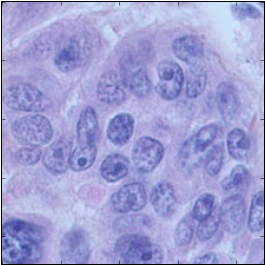
\includegraphics[height=3.0cm]{RGB_pred}}
%  \vspace{1.5cm}
  \centerline{Original RGB sample}\medskip
\end{minipage}
\hfill
\begin{minipage}[b]{0.48\linewidth}
  \centering
  \centerline{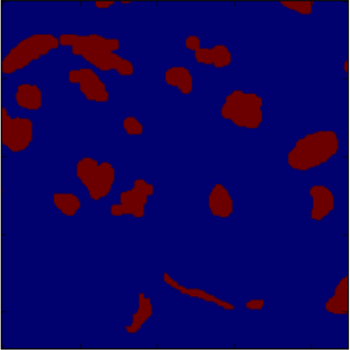
\includegraphics[width=3.0cm]{GT_pred}}
%  \vspace{1.5cm}
  \centerline{Associated ground truth}\medskip
\end{minipage}


\begin{minipage}[b]{0.32\linewidth}
  \centering
  \centerline{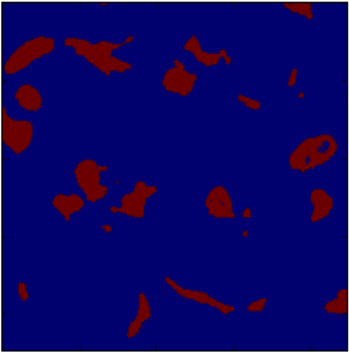
\includegraphics[height=2.4cm]{BaochuanB}}
%  \vspace{1.5cm}
  \centerline{PangNet}\medskip
\end{minipage}
\hfill
\begin{minipage}[b]{.32\linewidth}
  \centering
  \centerline{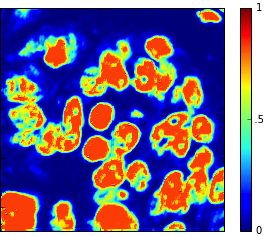
\includegraphics[height=2.5cm]{BaochuanP}}
%  \vspace{1.5cm}
  \centerline{Probability map}\medskip
\end{minipage}
\hfill
\begin{minipage}[b]{.32\linewidth}
  \centering
  \centerline{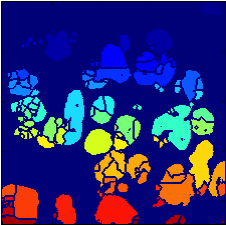
\includegraphics[height=2.4cm]{Baochuan_WS}}
%  \vspace{1.5cm}
  \centerline{Watershed}\medskip
\end{minipage}

%
%
\begin{minipage}[b]{0.32\linewidth}
  \centering
  \centerline{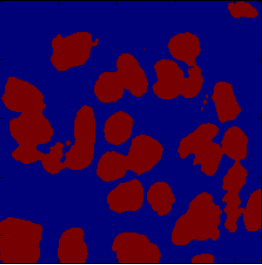
\includegraphics[height=2.4cm]{DeconvNetB}}
%  \vspace{1.5cm}
  \centerline{DeconvNet}\medskip
\end{minipage}
\hfill
\begin{minipage}[b]{.32\linewidth}
  \centering
  \centerline{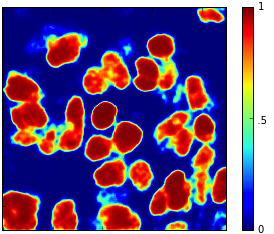
\includegraphics[height=2.4cm]{DeconvNetP}}
%  \vspace{1.5cm}
  \centerline{Probability map}\medskip
\end{minipage}
\hfill
\begin{minipage}[b]{.32\linewidth}
  \centering
  \centerline{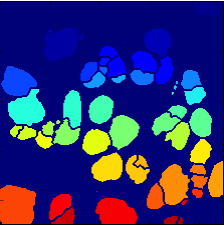
\includegraphics[height=2.4cm]{DeconvNet_WS}}
%  \vspace{1.5cm}
  \centerline{Watershed}\medskip
\end{minipage}
%
\begin{minipage}[b]{0.32\linewidth}
  \centering
  \centerline{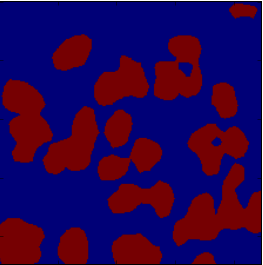
\includegraphics[height=2.4cm]{FCNB}}
%  \vspace{1.5cm}
  \centerline{FCN}\medskip
\end{minipage}
\hfill
\begin{minipage}[b]{.32\linewidth}
  \centering
  \centerline{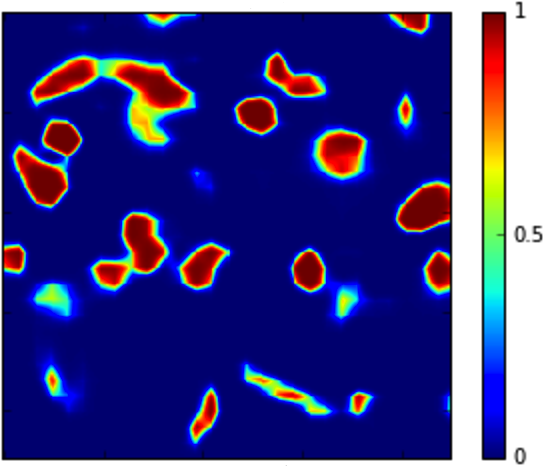
\includegraphics[height=2.4cm]{FCNP}}
%  \vspace{1.5cm}
  \centerline{Probability map}\medskip
\end{minipage}
\hfill
\begin{minipage}[b]{.32\linewidth}
  \centering
  \centerline{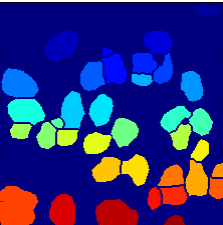
\includegraphics[height=2.4cm]{FCN_WS}}
%  \vspace{1.5cm}
  \centerline{Watershed}\medskip
\end{minipage}

%\begin{minipage}[b]{0.32\linewidth}
%  \centering
%  \centerline{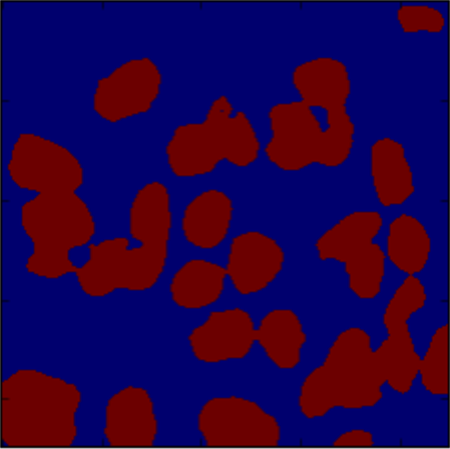
\includegraphics[height=2.4cm]{EnsembleB}}
%%  \vspace{1.5cm}
%  \centerline{Ensemble}\medskip
%\end{minipage}
%\hfill
%\begin{minipage}[b]{.32\linewidth}
%  \centering
%  \centerline{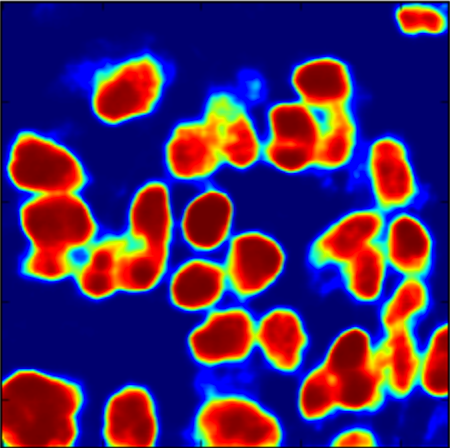
\includegraphics[height=2.4cm]{EnsembleP}}
%%  \vspace{1.5cm}
%  \centerline{Probability map}\medskip
%\end{minipage}
%\hfill
%\begin{minipage}[b]{.32\linewidth}
%  \centering
%  \centerline{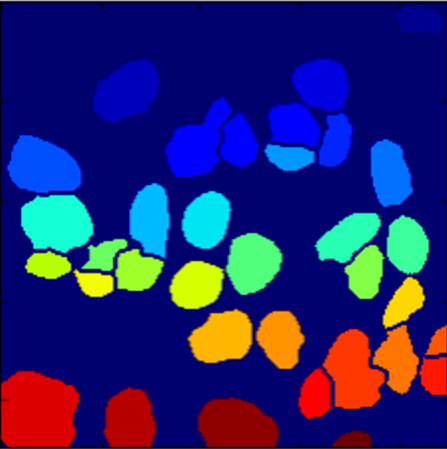
\includegraphics[height=2.4cm]{Ensemble_WS}}
%%  \vspace{1.5cm}
%  \centerline{Watershed}\medskip
%\end{minipage}

%
\caption{Prediction via different classifiers of a random sample on the left out patient: 581910}
\label{fig:prediction}
%
\end{figure}

%depending on the morphological dynamic at the moment at which two
%regions get in contact. 
%This algorithm will be made publicly available
%through the open-source software scikit-image\cite{scikit-image}, in which we implemented
%all the steps which were not related to deep learning. 



\section{Different architectures}
\label{sec:results}
\noindent We experience with 3 known arhitectures in semantic segmentation, named PangNet, Fully Convolutionnal Net (FCN) and DeconvNet. The most basic architecture, PangNet, consists of 4 
convolutionnal layer where each convolutionnal layer has 8 feature map, for more information please refer to \cite{pang2010cell}. 
This net, being not deep, has the advantage of being less 
computationnally intensive. FCN is a first attempt of applying "deep 
feature" representations to the task of semantic segmentation. This 
architecture has the advantage of re-using a classical deep learning 
architecture with additional upsampling and skip layers. The 
upsampling layers enable the network to learn a pixel level classification 
and the skip layers enable the network to fuse different levels of 
abstraction to the final prediction. This model can be fine tuned with a 
set of pretrained-weights extracted from the classical deep learning 
architecture\cite{long2015fcn}. DeconvNet is also based on a classical architecture, 
however, in this network their are no skip layers as one intends to learn 
the proper upsampling through repeated deconvolution and convolution 
layers. This model can also be fine tuned\cite{noh2015learning}. We also did an
ensemble classifier of these two previous nets as suggested in 
\cite{noh2015learning} but did not include any illustration as the results of the FCN were better.

\section{Results and discussion}
\label{sec:result}
\noindent We conducted our experiments on GPUs via the caffe framework, 
\cite{jia2014caffe}. We present our results in table \ref{tab:res} where 
we averaged the metrics over all left out patients. We also added, for 
illustration purposes \ref{fig:prediction}, image predictions and 
associated 
probability maps to evaluate some differences between the classifiers. 
We notice that the simpler net, PangNet seems to have learnt simple 
rules such as color information. As soon as the nuclei are not
homogeneous and dark inside, the method fails ( "holes" in the
cells). On the 
contrary, deeper nets as FCN and DeconvNet have learnt deeper features 
and seem capable of recognizing whole cells. On these probability maps 
we applied our watershed segmentation and we can picture the results in 
the third 
column. By construction, our post-processing 
scheme is very sensitive to noise as we can see in the PangNet 
prediction, many unrelated minimas will lead to highly partitionned cell. 
This phenomenom also appears with the DeconvNet where undesired 
cuts were performed, like for the cell at the bottom left of the image. 
We picked $\lambda = 7$ which seemed to give a nice partitionning of 
the image, this value can be found by cross validation.
\begin{table}
\begin{tabular}{|c|c|c|c|c|}
\hline
  & PangNet & DeconvNet & FCN & Ensemble\\
 \hline
Accuracy  &       0.936 & 0.968 &0.958 & 0.968  \\
IU   &    0.759 &     0.856 & 0.857 & 0.861 \\
Recall     &       0.744  &     0.856 & 0.855 & 0.876\\
Precision   &       0.741 &     0.858 & 0.878 & 0.851\\
F1    &       0.742 &     0.856 & 0.866  & 0.863\\
% TP       &       0.744 &     0.856 & 0.855 & 0.876 \\
% TN      &       0.963 &     0.981 &  0.977 & 0.979\\
Performance    &       0.853 &     0.918 & 0.916 & 0.928\\
% Pixel error  &  0.063 &     0.032 & 0.042 & 0.032\\
\hline
\end{tabular}
\caption{Results}
\label{tab:res}
\end{table}

\section{Conclusion}
\label{sec:conclusion}

\noindent We presented a fully automized workflow for segmenting nuclei in
histopathology images based on deep learning and mathematical
morphology. We have also generated a manually curated segmentation
data base, which we make publicly available. We believe that such a
method can become very useful for the investigation of cellular
phenotypes at a tissue level and their relation to disease. 

%%with Unet
%\begin{tabular}{|c|c|c|c|c|c|}
% & UNet & PangNet & DeconvNet & FCN & Ensemble \\
%\hrule
%Accuracy &       0.89 &       0.936 & 0.968 &0.958 & \\
%IU   &       0.70 &       0.759 &     0.856 & 0.857 &\\
%Recall    &       0.75 &       0.744  &     0.856 & 0.855 &\\
%Precision    &       0.64 &       0.741 &     0.858 & 0.878&\\
%F1       &       0.69 &       0.742 &     0.856 & 0.866&  \\
%TP             &       0.75 &       0.744 &     0.856 & 0.855 & \\
%TN             &       0.92 &       0.963 &     0.981 &  0.977&\\
%Performance    &       0.84 &       0.853 &     0.918 & 0.916&\\
%Pixel error  &       0.11 &       0.063 &     0.032 & 0.042&\\
%\end{tabular}
\bibliographystyle{IEEEbib}
\bibliography{refs}

\end{document}
